\begin{figure}[H]
    \centering
    \caption{the priority of items after request to D}
    \label{fig:my_label}
\newcounter{row2}
\newcounter{col2}

\newcommand\setrows[4]{
  \setcounter{col2}{1}
  \foreach \n in {#1, #2, #3, #4} {
    \edef\x{\value{col2} - 0.5}
    \edef\y{7.5 - \value{row2}}
    \node[anchor=center] at (\x, \y) {\n};
    \stepcounter{col2}
  }
  \stepcounter{row2}
}
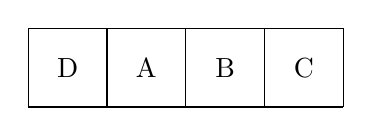
\begin{tikzpicture}[scale=1]

\begin{scope}
\draw (0, 0) grid (4, 1);
\draw[very thin] (0, 0) grid (4, 1);
\setcounter{row2}{7}
\setrows{D}{A}{B}{C}
\end{scope}
\end{tikzpicture}
\\
and compare it to the caches of sizes 3 and 4
\\
\begin{tikzpicture}
        \node[rounded corners,draw=black,minimum size=2cm, label=above: cache size 4] (o) at (0,0)  { 
    \begin{tikzpicture}
        \node[rounded corners,draw=black,minimum size=0.8cm]{A};
    \end{tikzpicture}
    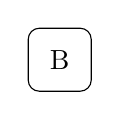
\begin{tikzpicture}
        \node[rounded corners,draw=black,minimum size=0.8cm]{B};
    \end{tikzpicture}
    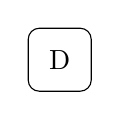
\begin{tikzpicture}
        \node[rounded corners,draw=black,minimum size=0.8cm]{D};
    \end{tikzpicture}
    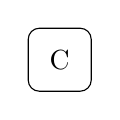
\begin{tikzpicture}
        \node[rounded corners,draw=black,minimum size=0.8cm]{C};
    \end{tikzpicture}
    };  
        \node[rounded corners,draw=black,minimum size=2cm,label=above: cache size 3] (o) at (5,0)  { 
    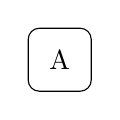
\begin{tikzpicture}
        \node[rounded corners,draw=black,minimum size=0.8cm]{A};
    \end{tikzpicture}
    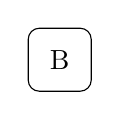
\begin{tikzpicture}
        \node[rounded corners,draw=black,minimum size=0.8cm]{B};
    \end{tikzpicture}
    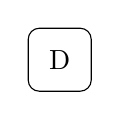
\begin{tikzpicture}
        \node[rounded corners,draw=black,minimum size=0.8cm]{D};
    \end{tikzpicture}
    };  
\end{tikzpicture}
\end{figure}
